\section{Pooling}
\textbf{MaxPooling1D:} 1 boyutlu veriler üzerinde maksimum havuzlama işlemi uygulamak için kullanılır. Giriş verilerinin boyutunu küçültmek ve önemli özellikleri vurgulamak için kullanılır. Belirli bir pencere boyutunda giriş verileri üzerinde kaydırılan bir pencereyi kullanarak maksimum havuzlama işlemi uygular. Bu işlem, her pencere üzerindeki en büyük değeri alarak giriş verisinin boyutunu küçültür.\\
\textbf{AveragePooling1D:} 1 boyutlu verileri üzerinde ortalama havuzlama işlemi uygulamak için kullanılır. Belirli bir pencere boyutunda giriş verileri üzerinde kaydırılan bir pencereyi kullanarak ortalama havuzlama işlemi uygular. Her pencere üzerindeki değerlerin ortalamasını alarak giriş verisinin boyutunu küçültür.\\
\textbf{GlobalMaxPooling1D:} 1 boyutlu veriler üzerinde global maksimum havuzlama işlemi uygulamak için kullanılır. Bu katman, giriş verilerinin tüm zaman adımları boyunca maksimum değerini alarak giriş verisinin boyutunu azaltır ve önemli özellikleri vurgular.\\
\textbf{GlobalAveragePooling1D:} 1 boyutlu veriler üzerinde global ortalama havuzlama işlemi uygulamak için kullanılır. Bu katman, giriş verilerinin tüm zaman adımları boyunca ortalama değerini alarak giriş verisinin boyutunu azaltır ve önemli özellikleri vurgular.

\begin{figure}[h]
    \centering
    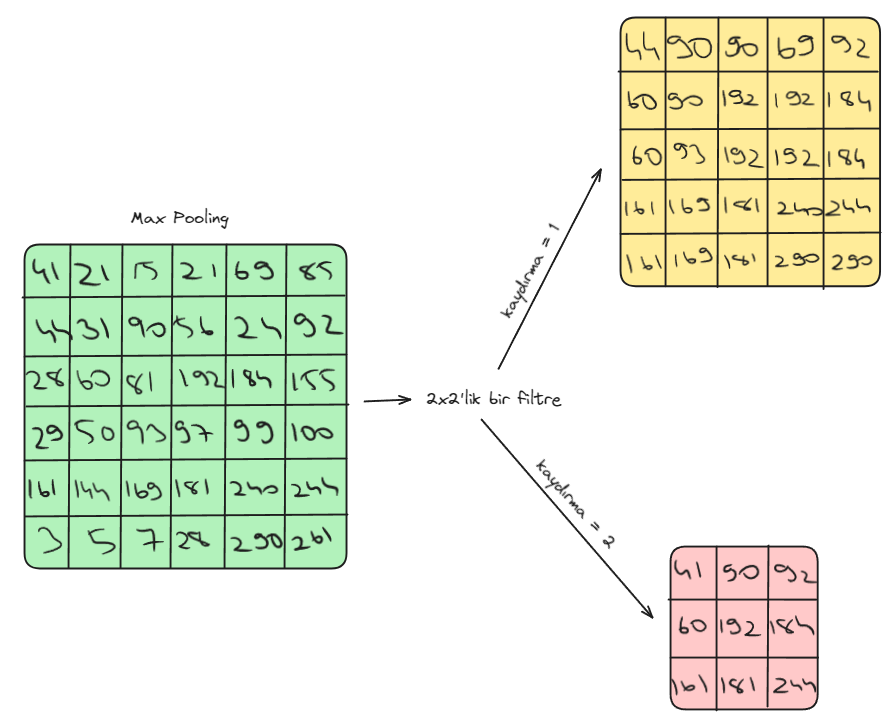
\includegraphics[width=0.7\textwidth]{images/pooling_layer.png}
    \caption{Pooling katmanı.}
    \label{fig:enter-label}
\end{figure}

\newpage